% Options for packages loaded elsewhere
\PassOptionsToPackage{unicode}{hyperref}
\PassOptionsToPackage{hyphens}{url}
\PassOptionsToPackage{dvipsnames,svgnames,x11names}{xcolor}
%
\documentclass[
]{book}
\usepackage{amsmath,amssymb}
\usepackage{lmodern}
\usepackage{iftex}
\ifPDFTeX
  \usepackage[T1]{fontenc}
  \usepackage[utf8]{inputenc}
  \usepackage{textcomp} % provide euro and other symbols
\else % if luatex or xetex
  \usepackage{unicode-math}
  \defaultfontfeatures{Scale=MatchLowercase}
  \defaultfontfeatures[\rmfamily]{Ligatures=TeX,Scale=1}
\fi
% Use upquote if available, for straight quotes in verbatim environments
\IfFileExists{upquote.sty}{\usepackage{upquote}}{}
\IfFileExists{microtype.sty}{% use microtype if available
  \usepackage[]{microtype}
  \UseMicrotypeSet[protrusion]{basicmath} % disable protrusion for tt fonts
}{}
\makeatletter
\@ifundefined{KOMAClassName}{% if non-KOMA class
  \IfFileExists{parskip.sty}{%
    \usepackage{parskip}
  }{% else
    \setlength{\parindent}{0pt}
    \setlength{\parskip}{6pt plus 2pt minus 1pt}}
}{% if KOMA class
  \KOMAoptions{parskip=half}}
\makeatother
\usepackage{xcolor}
\IfFileExists{xurl.sty}{\usepackage{xurl}}{} % add URL line breaks if available
\IfFileExists{bookmark.sty}{\usepackage{bookmark}}{\usepackage{hyperref}}
\hypersetup{
  pdftitle={w203: Statistics for Data Science},
  pdfauthor={w203 Instructors},
  colorlinks=true,
  linkcolor={Maroon},
  filecolor={Maroon},
  citecolor={Blue},
  urlcolor={Blue},
  pdfcreator={LaTeX via pandoc}}
\urlstyle{same} % disable monospaced font for URLs
\usepackage{longtable,booktabs,array}
\usepackage{calc} % for calculating minipage widths
% Correct order of tables after \paragraph or \subparagraph
\usepackage{etoolbox}
\makeatletter
\patchcmd\longtable{\par}{\if@noskipsec\mbox{}\fi\par}{}{}
\makeatother
% Allow footnotes in longtable head/foot
\IfFileExists{footnotehyper.sty}{\usepackage{footnotehyper}}{\usepackage{footnote}}
\makesavenoteenv{longtable}
\usepackage{graphicx}
\makeatletter
\def\maxwidth{\ifdim\Gin@nat@width>\linewidth\linewidth\else\Gin@nat@width\fi}
\def\maxheight{\ifdim\Gin@nat@height>\textheight\textheight\else\Gin@nat@height\fi}
\makeatother
% Scale images if necessary, so that they will not overflow the page
% margins by default, and it is still possible to overwrite the defaults
% using explicit options in \includegraphics[width, height, ...]{}
\setkeys{Gin}{width=\maxwidth,height=\maxheight,keepaspectratio}
% Set default figure placement to htbp
\makeatletter
\def\fps@figure{htbp}
\makeatother
\setlength{\emergencystretch}{3em} % prevent overfull lines
\providecommand{\tightlist}{%
  \setlength{\itemsep}{0pt}\setlength{\parskip}{0pt}}
\setcounter{secnumdepth}{5}
\usepackage{charter}
\usepackage{euler}
\ifLuaTeX
  \usepackage{selnolig}  % disable illegal ligatures
\fi
\usepackage[]{natbib}
\bibliographystyle{apalike}

\title{w203: Statistics for Data Science}
\author{w203 Instructors}
\date{2022-02-10}

\usepackage{amsthm}
\newtheorem{theorem}{Theorem}[chapter]
\newtheorem{lemma}{Lemma}[chapter]
\newtheorem{corollary}{Corollary}[chapter]
\newtheorem{proposition}{Proposition}[chapter]
\newtheorem{conjecture}{Conjecture}[chapter]
\theoremstyle{definition}
\newtheorem{definition}{Definition}[chapter]
\theoremstyle{definition}
\newtheorem{example}{Example}[chapter]
\theoremstyle{definition}
\newtheorem{exercise}{Exercise}[chapter]
\theoremstyle{definition}
\newtheorem{hypothesis}{Hypothesis}[chapter]
\theoremstyle{remark}
\newtheorem*{remark}{Remark}
\newtheorem*{solution}{Solution}
\begin{document}
\maketitle

{
\hypersetup{linkcolor=}
\setcounter{tocdepth}{1}
\tableofcontents
}
\newcommand{\E}[1]{{\mathbb{E}\left[ #1 \right]}}
\newcommand{\V}[1]{{\mathbb{V}\left[ #1 \right]}}
\newcommand{\C}[1]{{\text{Cov}\left[ #1 \right]}}
\newcommand{\v}[1]{{\boldsymbol{#1}}}
\newcommand{\m}[1]{{\mathbb{#1}}}

\hypertarget{cover}{%
\chapter*{Cover}\label{cover}}
\addcontentsline{toc}{chapter}{Cover}

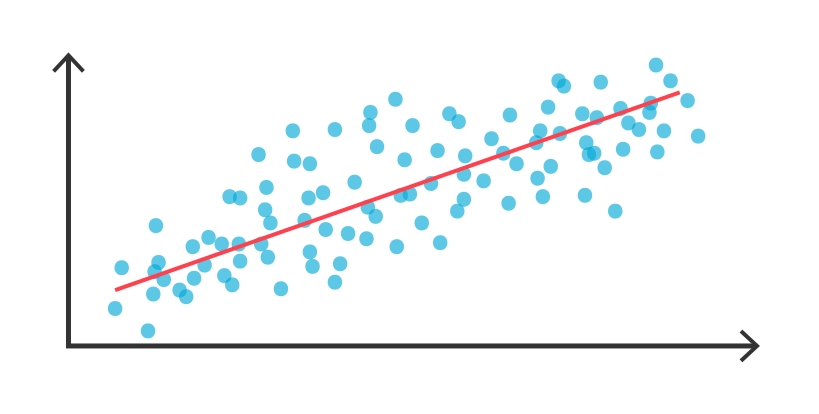
\includegraphics[width=0.85\linewidth]{./images/cover}

\hypertarget{part-probability-theory}{%
\part{Probability Theory}\label{part-probability-theory}}

\hypertarget{probability-spaces}{%
\chapter{Probability Spaces}\label{probability-spaces}}

\hypertarget{kolmogorovs-axioms}{%
\section{Kolmogorov's Axioms}\label{kolmogorovs-axioms}}

\hypertarget{conditional-probability}{%
\section{Conditional Probability}\label{conditional-probability}}

\hypertarget{random-variables}{%
\chapter{Random Variables}\label{random-variables}}

\hypertarget{part-learning-from-data}{%
\part{Learning from Data}\label{part-learning-from-data}}

\hypertarget{hypothesis-testing}{%
\chapter{Hypothesis Testing}\label{hypothesis-testing}}

\hypertarget{regression}{%
\chapter{Regression}\label{regression}}

We write a \(k\)-vector (of scalars) as
\[
{\boldsymbol{x}}=
\begin{bmatrix}
x_1 \\
x_2 \\
\vdots \\
x_k
\end{bmatrix}
\]
The transpose of \({\boldsymbol{x}}\) as
\[
{\boldsymbol{x}}^T=
\begin{bmatrix}
x_1 & x_2 & \ldots & x_k
\end{bmatrix}.
\]
We use uppercase letters \(X,Y,Z,\ldots\) to denote random variables. Random vectors are denoted by \textbf{bold} uppercase letters \({\boldsymbol{X}},{\boldsymbol{Y}},{\boldsymbol{Z}},\ldots\), and written as a column vector. For example, \[
{\boldsymbol{X}}=
\begin{bmatrix}
X_{[1]}\\
X_{[2]}\\
\vdots \\
X_{[k]} \\
\end{bmatrix}_{k\times 1}
\]
In order to distinguish random matrices from vectors, a random matrix is denoted by \({\mathbb{X}}\).

The expectation of \({\boldsymbol{X}}\) is defined as
\[
{\mathbb{E}}[{\boldsymbol{X}}]=
\begin{bmatrix}
{\mathbb{E}\left[ X_{[1]} \right]} \\
{\mathbb{E}\left[ X_{[2]} \right]} \\
\vdots \\
{\mathbb{E}\left[ X_{[k]} \right]} \\
\end{bmatrix}
\]
The \(k\times k\) covariance matrix of \({\boldsymbol{X}}\) is defined as
\[
\begin{aligned}
{\mathbb{V}\left[ {\boldsymbol{X}} \right]} &={\mathbb{E}\left[ ({\boldsymbol{X}}-{\mathbb{E}\left[ {\boldsymbol{X}} \right]})({\boldsymbol{X}}-{\mathbb{E}\left[ {\boldsymbol{X}} \right]})^T \right]} \\
&=\begin{bmatrix}
\sigma_1^2 & \sigma_{12} & \ldots & \sigma_{1k} \\
\sigma_{21} & \sigma_{2}^2 & \ldots & \sigma_{2k} \\
\vdots & \vdots & \ddots & \vdots \\
\sigma_{k1} & \sigma_{k2}^2 & \ldots & \sigma_{k}^2 \\
\end{bmatrix}_{k\times k}
\end{aligned}
\]

where \(\sigma_j={\mathbb{V}\left[ X_{[j]} \right]}\) and \(\sigma_{ij}={\text{Cov}\left[ X_{[i]},X_{[j]} \right]}\) for \(i,j=1,2,\ldots,k\) and \(i\neq j\).

\begin{theorem}[Linearity of Exectation]
\protect\hypertarget{thm:explin}{}\label{thm:explin}Let \({\mathbb{A}}_{l\times k},{\mathbb{B}}_{m\times l}\) be fixed matrices and \({\boldsymbol{c}}\) a fixed vector of size \(l\). If \({\boldsymbol{X}}\) and \({\boldsymbol{Y}}\) are random vectors of size \(k\) and \(m\), respectively, such that \({\mathbb{E}\left[ X \right]}<\infty,{\mathbb{E}\left[ Y \right]}<\infty\), then
\[
{\mathbb{E}\left[ {\mathbb{A}}{\boldsymbol{X}}+{\boldsymbol{Y}}{\mathbb{B}}+{\boldsymbol{c}} \right]}={\mathbb{A}}{\mathbb{E}\left[ {\boldsymbol{X}} \right]}+{\mathbb{E}\left[ {\boldsymbol{Y}} \right]}{\mathbb{B}}+{\boldsymbol{c}}.
\]
\end{theorem}

\hypertarget{conditional-expectation-function}{%
\section{Conditional Expectation Function}\label{conditional-expectation-function}}

\begin{theorem}[Characterization of CEF]
\protect\hypertarget{thm:cef}{}\label{thm:cef}If ~\({\mathbb{E}\left[ Y^2 \right]}<\infty\) and \({\boldsymbol{X}}\) is a random vector such that \(Y=m({\boldsymbol{X}})+e\), then the following statements are equivalent:\\
1. \(m({\boldsymbol{X}})={\mathbb{E}\left[ Y|{\boldsymbol{X}} \right]}\), the CEF of \(Y\) given \({\boldsymbol{X}}\)\\
2. \({\mathbb{E}\left[ e|{\boldsymbol{X}} \right]}=0\)
\end{theorem}

\hypertarget{best-linear-predictor}{%
\section{Best Linear Predictor}\label{best-linear-predictor}}

Let \(Y\) be a random variable and \({\boldsymbol{X}}\) be a random vector. We denote the \textbf{best linear predictor} of \(Y\) given \({\boldsymbol{X}}\) by \(\mathscr{P}[Y|{\boldsymbol{X}}]\). It's also called the \textbf{linear projection} of \(Y\) on \({\boldsymbol{X}}\).

\begin{theorem}[Best Linear Predictor]
\protect\hypertarget{thm:blp}{}\label{thm:blp}Under the following assumptions

\begin{enumerate}
\def\labelenumi{\arabic{enumi}.}
\tightlist
\item
  \({\mathbb{E}\left[ Y^2 \right]}<\infty\)
\item
  \({\mathbb{E}\left[ ||\bf{X}||^2 \right]}<\infty\)
\item
  \({\mathbb{Q}}_{\bf{XX}}\stackrel{\text{def}}{=}{\mathbb{E}\left[ {\boldsymbol{X}}{\boldsymbol{X}}^T \right]}\) is positive-definite
\end{enumerate}

the best linear predictor exists uniquely, and has the form
\[
\mathscr{P}[Y|{\boldsymbol{X}}]={\boldsymbol{X}}^T{\boldsymbol{\beta}},
\]
where \({\boldsymbol{\beta}}=\left({\mathbb{E}\left[ {\boldsymbol{X}}{\boldsymbol{X}}^T \right]}\right)^{-1}{\mathbb{E}}[{\boldsymbol{X}}Y]\).
\end{theorem}

\begin{theorem}[Best Linear Predictor Error]
\protect\hypertarget{thm:blperror}{}\label{thm:blperror}

If the BLP exists, the linear projection error \(e=Y-\mathscr{P}[Y|{\boldsymbol{X}}]\) follows the following properties:

\begin{enumerate}
\def\labelenumi{\arabic{enumi}.}
\tightlist
\item
  \({\mathbb{E}}[{\boldsymbol{X}}e]={\boldsymbol{0}}\)
\item
  \({\mathbb{E}}[e]=0\) if
  \({\boldsymbol{X}}'=\begin{bmatrix}1 & X_1 & \ldots & X_k \end{bmatrix}\).
\end{enumerate}

\end{theorem}

\hypertarget{ordinary-least-squares}{%
\chapter{Ordinary Least Squares}\label{ordinary-least-squares}}

Let \(Y\) be our outcome random variable and
\[
\pmb{X}=\begin{bmatrix}
1 \\ X_1 \\ X_2 \\ \vdots \\ X_k
\end{bmatrix}_{(k+1)\times 1}
\]
be our predictor vector containing \(k\) predictors and a constant. We denote the joint distribution of \((Y,\pmb{X})\) by \(F(y,\pmb{x})\), i.e.,
\[
F(y,\pmb{x})=\mathbb{P}(Y\leq y, \pmb{X}\leq\pmb{x})
=\mathbb{P}(Y\leq y,X_1\leq x_1,\ldots,X_k\leq x_k).
\]

The \textbf{dataset} or \textbf{sample} is a collection of observations \(\{(Y_i,\pmb{X}_i): i=1,2,\ldots,n\}\). We assume that each observation
\((Y_i,\pmb{X}_i)\) is a random vector drawn from the common distribution or \textbf{population} \(F\).

\hypertarget{matrix-formulation}{%
\section{Matrix Formulation}\label{matrix-formulation}}

For a given vector of (unknown) coefficients
\(\pmb{\beta}=\begin{bmatrix}\beta_0 & \beta_1 & \ldots & \beta_k\end{bmatrix}'\in\mathbb{R}^{k+1}\), we define the following \textbf{cost function}:
\[
\widehat{S}(\pmb{\beta})=\frac{1}{n}\sum\limits_{i=1}^n(Y_i-\pmb{X_i}'\pmb{\beta})^2.
\]
The cost function \(\widehat{S}({\pmb{\beta}})\) can also be thought of as the average sum of residuals. In fact, \(\widehat{S}({\pmb{\beta}})\) is the moment (plug-in) estimator of the mean squared error,
\[
S(\pmb{\beta})={\mathbb{E}\left[ (Y-\pmb{X}'\pmb{\beta})^2 \right]}.
\]

We now minimize \(\widehat{S}({\pmb{\beta}})\) over all possible choices of
\(\pmb{\beta}\in\mathbb{R}^{k+1}\). When the minimizer exists and is unique, we call it the \textbf{least squares estimator}, denoted \(\widehat{\pmb{\beta}}\).

\begin{definition}[(Ordinary) Least Squares Estimator]
The least square estimator is \[
\widehat{\pmb{\beta}}
=\underset{\pmb{\beta}\in\mathbb{R}^{k+1}}{\arg\min} \ \widehat{S}(\pmb{\beta}),
\]
provided it exists uniquely.
\end{definition}

\hypertarget{solution-of-ols}{%
\section{Solution of OLS}\label{solution-of-ols}}

We rewrite the cost function as
\[
\widehat{S}(\pmb{\beta})=\frac{1}{n}SSE(\pmb{\beta}),
\]
where
\(SSE(\pmb{\beta}):=\sum\limits_{i=1}^n(Y_i-\pmb{X_i}'\pmb{\beta})^2\).

We now express \(SSE(\pmb{\beta})\) as a quadratic function of \(\pmb{\beta}'\).
\begin{align}
SSE &=\sum\limits_{i=1}^n(Y_i-\pmb{X_i}'\pmb{\beta})^2 \\
&=\sum\limits_{i=1}^n Y_i^2 
  - 2\sum\limits_{i=1}^n Y_i(\pmb{X_i}'\pmb{\beta})
  + \sum\limits_{i=1}^n (\pmb{X_i}'\pmb{\beta})^2 \\
&=\sum\limits_{i=1}^n Y_i^2 
  - 2\sum\limits_{i=1}^n Y_i(\pmb{\beta}'\pmb{X_i})
  + \sum\limits_{i=1}^n (\pmb{X_i}'\pmb{\beta})(\pmb{X_i}'\pmb{\beta}) \\
&=\sum\limits_{i=1}^n Y_i^2 
  - 2\sum\limits_{i=1}^n \pmb{\beta}'(Y_i\pmb{X_i})
  + \sum\limits_{i=1}^n (\pmb{\beta}'\pmb{X_i})(\pmb{X_i}'\pmb{\beta}) \\
&=\left(\sum\limits_{i=1}^n Y_i^2\right) 
  - 2\pmb{\beta}'\left(\sum\limits_{i=1}^n\pmb{X_i}Y_i\right)
  + \pmb{\beta}'\left(\sum\limits_{i=1}^n \pmb{X_i}\pmb{X_i}'\right)\pmb{\beta}
\end{align}
Taking partial derivative w.r.t. \(\beta_j\), we get
\[
\frac{\partial}{\partial\beta_j}SSE(\pmb{\beta})=-2\left[\sum\limits_{i=1}^n\pmb{X_i}Y_i\right]_j 
+ 2\left[\left(\sum\limits_{i=1}^n  \pmb{X_i}\pmb{X_i}'\right)\pmb{\beta}\right]_j.
\]

Therefore,
\[
\frac{\partial}{\partial\pmb{\beta}}SSE(\pmb{\beta})
=-2\left(\sum\limits_{i=1}^n\pmb{X_i}Y_i\right) 
+ 2\left(\sum\limits_{i=1}^n  \pmb{X_i}\pmb{X_i}'\right)\pmb{\beta}.
\]

In order to miniminize \(SSE(\pmb{\beta})\), a necessary condition for \(\widehat{\pmb{\beta}}\) is
\[
\frac{\partial}{\partial\pmb{\beta}}SSE(\pmb{\beta})\bigg|_{\pmb{\beta}
=\widehat{\pmb{\beta}}}=\pmb{0},
\]
i.e.,
\[
-2\left(\sum\limits_{i=1}^n\pmb{X_i}Y_i\right) 
+ 2\left(\sum\limits_{i=1}^n  \pmb{X_i}\pmb{X_i}'\right)\widehat{\pmb{\beta}}
=\pmb{0}
\]
So,
\begin{equation}
\left(\sum\limits_{i=1}^n\pmb{X_i}Y_i\right)
=\left(\sum\limits_{i=1}^n  \pmb{X_i}\pmb{X_i}'\right)\widehat{\pmb{\beta}}
\label{eq:moment-0}
\end{equation}

Both the left and right hand side of the above equation are \(k+1\) vectors. So, we have a system of \((k+1)\) linear equations with \((k+1)\) unknowns---the elements of \(\pmb{\beta}\).

Let us define

\[
\widehat{\mathbb{Q}}_{\pmb{XX}}
=\frac{1}{n}\left(\sum\limits_{i=1}^n\pmb{X_i}\pmb{X_i}'\right)
\mbox{ and }
\widehat{\mathbb{Q}}_{\pmb{X}Y}
=\frac{1}{n}\left(\sum\limits_{i=1}^n\pmb{X_i}Y_i\right).
\]

Rewriting \eqref{eq:moment-0}, we get
\begin{equation}
\widehat{\mathbb{Q}}_{\pmb{X}Y}=\widehat{\mathbb{Q}}_{\pmb{XX}}
\widehat{\pmb{\beta}}.
\label{eq:moment}
\end{equation}

Equation \eqref{eq:moment} is sometimes referred to as the first-order moment condition. For the uniqueness of solution, we require that
\(\widehat{\mathbb{Q}}_{\pmb{XX}}\) is non-singular. In that case, we can solve for \(\widehat{\pmb{\beta}}\) to get,
\[
\widehat{\pmb{\beta}}=\left[\widehat{\mathbb{Q}}_{\pmb{XX}}\right]^{-1}
\widehat{\mathbb{Q}}_{\pmb{X}Y}.
\]
To verify that the above choice minimizes \(SSE(\pmb{\beta})\),
one can consider the second-order moment conditions.
\[
\frac{\partial^2}{\partial\pmb{\beta}\partial\pmb{\beta}'}SSE(\pmb{\beta})
=2\widehat{\mathbb{Q}}_{\pmb{XX}}.
\]
If \(\widehat{\mathbb{Q}}_{\pmb{XX}}\) is non-singular, it is also positive-definite. So, we have actually proved the following theorem.

\begin{theorem}
If ~\(\widehat{\mathbb{Q}}_{\pmb{XX}}\) is non-singular, then the
least squares estimator is unique, and is given by
\[
\widehat{\pmb{\beta}}=\left[\widehat{\mathbb{Q}}_{\pmb{XX}}\right]^{-1}
\widehat{\mathbb{Q}}_{\pmb{X}Y}.
\]
\end{theorem}

\hypertarget{errors-and-residuals}{%
\section{Errors and Residuals}\label{errors-and-residuals}}

We first define the \textbf{fitted} value as
\[
\widehat{Y}_i=\pmb{X}_i'\widehat{\pmb{\beta}}\mbox{ for }
i=1,2,\ldots,n.
\]
For the least squares estimators, we define the \textbf{errors} and \textbf{residuals} in the following way:
\[
e_i=Y_i-\pmb{X}'\pmb{\beta}, \mbox{ and } 
\widehat{e}_i=Y_i-\widehat{Y}_i.
\]

\begin{theorem}[Least Squares Error]
\protect\hypertarget{thm:olserror}{}\label{thm:olserror}If ~\(\widehat{\mathbb{Q}}_{\pmb{XX}}\) is non-singular, then\\
1. \(\sum\limits_{i=1}^n\pmb{X}_i\widehat{e}_i=\pmb{0}\)\\
2. \(\sum\limits_{i=1}^n\widehat{e}_i=0\)
\end{theorem}

\begin{proof}
\begin{align}
\sum\limits_{i=1}^n\pmb{X}_i\widehat{e}_i 
&=\sum\limits_{i=1}^n\pmb{X}_i(Y_i-\widehat{Y}_i) \\
&=\sum\limits_{i=1}^n\pmb{X}_iY_i-\sum\limits_{i=1}^n\pmb{X}_i\widehat{Y}_i \\
&=\sum\limits_{i=1}^n\pmb{X}_iY_i-\sum\limits_{i=1}^n\pmb{X}_i\pmb{X}_i'\pmb{\widehat{\beta}} \\
&=\widehat{Q}_{\pmb{X}Y}-\widehat{Q}_{\pmb{XX}}\pmb{\widehat{\beta}} \\
&=\widehat{Q}_{\pmb{X}Y}-\widehat{Q}_{\pmb{XX}}
\left( \widehat{Q}_{\pmb{XX}}^{-1} \widehat{Q}_{\pmb{X}Y} \right) \\
&=\pmb{0}
\end{align}

From the first row of (1) we get

\[
\sum\limits_{i=1}^n X_{i1}\widehat{e}_i=0.
\]
Since \(X_{i1}=1\) for all \(i\), we have that
\[
\sum\limits_{i=1}^n\widehat{e}_i=0.
\]
Hence the result.
\end{proof}

\hypertarget{model-in-matrix-notation}{%
\section{Model in Matrix Notation}\label{model-in-matrix-notation}}

Taking the definition of errors from the last section, we can write down a system of \(n\) linear equations:
\begin{align}
Y_1 &= \pmb{X_1}'\pmb{\beta} + e_1 \\
Y_2 &= \pmb{X_2}'\pmb{\beta} + e_2 \\
& \vdots \\
Y_n &= \pmb{X_1}'\pmb{\beta} + e_n
\end{align}

Define
\[
\pmb{Y}=\begin{bmatrix}
Y_1 \\
Y_2 \\
\vdots \\
Y_n
\end{bmatrix}_{n\times1},\ 
\mathbb{X}=\begin{bmatrix}
\pmb{X}_1 \\
\pmb{X}_2 \\
\vdots \\
\pmb{X}_n
\end{bmatrix}_{n\times(k+1)}, \mbox{ and }
\pmb{e}=\begin{bmatrix}
e_1 \\
e_2 \\
\vdots \\
e_n
\end{bmatrix}_{n\times1}.
\]
We can now rewrite the system as the following:
\[
\pmb{Y}=\mathbb{X}\pmb{\beta}+\pmb{e}.
\]
Note that
\[
\mathbb{X}=\begin{bmatrix}
1 & X_{11} & X_{12} & \ldots & X_{1k} \\
1 & X_{21} & X_{22} & \ldots & X_{2k} \\
\vdots & \vdots & \vdots & \ddots & \vdots \\
1 & X_{n1} & X_{n2} & \ldots & X_{nk}
\end{bmatrix}
\]

We also note that
\[
\widehat{Q}_{\pmb{XX}}=\sum\limits_{i=1}^n\pmb{X}_i'\pmb{X}_i=
\mathbb{X}'\mathbb{X},
\]
and
\[
\widehat{Q}_{\pmb{X}Y}=\sum\limits_{i=1}^n\pmb{X}_iY_i=
\mathbb{X}'\pmb{Y}.
\]
So, we have write the least squares estimator as
\[
\widehat{\pmb{\beta}}=\left[\mathbb{X}'\mathbb{X}\right]^{-1}\mathbb{X}\pmb{Y}.
\]
Similarly, the residual vector is
\[
\widehat{\pmb{e}}=\pmb{Y}-\mathbb{X}\widehat{\pmb{\beta}}.
\]
As a consequence, we can write
\[
\mathbb{X}'\widehat{\pmb{e}}=\pmb{0}.
\]

\hypertarget{linear-conditional-expectation-function}{%
\chapter{Linear Conditional Expectation Function}\label{linear-conditional-expectation-function}}

\hypertarget{variance-of-error}{%
\section{Variance of Error}\label{variance-of-error}}

We first compute the (unconditional) variance of the error vector \(\pmb{e}\). The covariance matrix
\[
\mathbb{V}[\pmb{e}]={\mathbb{E}\left[ \pmb{e}\pmb{e}' \right]}-{\mathbb{E}\left[ \pmb{e} \right]}{\mathbb{E}\left[ \pmb{e}' \right]}={\mathbb{E}\left[ \pmb{e}\pmb{e}' \right]}\stackrel{\text{def}}{=}\mathbb{D}.
\]
For \(i\neq j\), the errors \(e_i\),\(e_j\) are independent. As a result, \({\mathbb{E}\left[ e_ie_j \right]}={\mathbb{E}\left[ e_i \right]}{\mathbb{E}\left[ e_j \right]}=0\). So, \(\mathbb{D}\) is a diagonal matrix with the \(i\)-th diagonal element \(\sigma_i^2\):
\[
\mathbb{D}=\begin{bmatrix}
\sigma_1^2 & 0 & \ldots & 0 \\
0 & \sigma_2^2 & \ldots & 0 \\
\vdots & \vdots & \ddots & \vdots \\
0 & 0 & \ldots & \sigma_n^2
\end{bmatrix}.
\]

\hypertarget{variance-of-ols-estimators}{%
\section{Variance of OLS Estimators}\label{variance-of-ols-estimators}}

\hypertarget{large-sample-regression}{%
\chapter{Large-Sample Regression}\label{large-sample-regression}}

We assume that the best linear predictor, \(\mathscr{P}[Y|\pmb{X}]\), of \(Y\) given \(\pmb{X}\) is \(\pmb{X}'\pmb{\beta}\). If we write
\[
Y=\pmb{X}'\pmb{\beta}+e.
\]
we have from Theorem \ref{thm:blperror}
\[{\mathbb{E}\left[ e \right]}=0,\mbox{ and }{\mathbb{E}\left[ \pmb{X}e \right]}=\pmb{0}.\]

We also assume that the dataset \(\{(Y_i,\pmb{X}_i)\}\) are taken \textbf{i.i.d.} from the joint distribution of \((Y,\pmb{X})\). For each \(i\), we can write
\[
Y_i=\pmb{X_i}'\pmb{\beta}+e_i.
\]
In matrix notation, we can write
\[
\pmb{Y}=\mathbb{X}'\pmb{\beta}+\pmb{e}.
\]
Then
\[{\mathbb{E}\left[ \pmb{e} \right]}=\pmb{0}\].

\hypertarget{consistency-of-ols-estimators}{%
\section{Consistency of OLS Estimators}\label{consistency-of-ols-estimators}}

\hypertarget{asymptotic-normality}{%
\section{Asymptotic Normality}\label{asymptotic-normality}}

We start by revealing an alternative expression for the OLS estimators \(\widehat{\pmb{\beta}}\) using matrix notation.
\begin{align}
\widehat{\pmb{\beta}}
&=\left[\mathbb{X}'\mathbb{X}\right]^{-1}\mathbb{X}'\pmb{Y} \\
&=\left[\mathbb{X}'\mathbb{X}\right]^{-1}\mathbb{X}'(\mathbb{X}\pmb{\beta}+\pmb{e}) \\
&=\left[\mathbb{X}'\mathbb{X}\right]^{-1}(\mathbb{X}'\mathbb{X})\pmb{\beta}+
\left[\mathbb{X}'\mathbb{X}\right]^{-1}\mathbb{X}'\pmb{e} \\
&=\pmb{\beta} + \left[\mathbb{X}'\mathbb{X}\right]^{-1}\mathbb{X}'\pmb{e}
\end{align}
So,
\begin{equation}
\widehat{\pmb{\beta}}-\pmb{\beta} = \left[\mathbb{X}'\mathbb{X}\right]^{-1}\mathbb{X}'\pmb{e}
\label{eq:beta}
\end{equation}

We can then multiply by \(\sqrt{n}\) both sides of Equation \eqref{eq:beta} to get
\begin{align}
\sqrt{n}\left(\widehat{\pmb{\beta}}-\pmb{\beta}\right)
&=\left( \frac{1}{n}\sum\limits_{i=1}^n\pmb{X}_i\pmb{X}_i' \right)^{-1}
\left( \frac{1}{\sqrt{n}}\sum\limits_{i=1}^n\pmb{X}_ie_i \right) \\
&=\widehat{\mathbb Q}_{\pmb{XX}}^{-1}
\left( \frac{1}{\sqrt{n}}\sum\limits_{i=1}^n\pmb{X}_ie_i \right)
\end{align}
From the consistency of OLS estimators, we already have
\[ \widehat{\mathbb Q}_{\pmb{XX}}\xrightarrow[p]{\quad\quad}\mathbb{Q}_{\pmb{XX}}\]
Our aim now is to understand the distribution of the stochastic term (the second term) in the above expression.

We first note (from i.i.d. and Theorem \ref{thm:blperror}) that
\[
{\mathbb{E}\left[ \pmb{X}_ie_i \right]}={\mathbb{E}\left[ \pmb{X}e \right]}=\pmb{0}.
\]
Let us compute the covariance matrix of \(\pmb{X}_ie_i\). Since the expectation vector is zero, we have
\[
\mathbb{V}[\pmb{X}_ie_i]={\mathbb{E}\left[ \pmb{X}_ie_i(\pmb{X}_ie_i)' \right]}={\mathbb{E}\left[ \pmb{X}e(\pmb{X}e)' \right]}={\mathbb{E}\left[ \pmb{X}\pmb{X}'e^2 \right]}\stackrel{\text{def}}{=}\mathbb{A}.
\]
As any function of \(\{(Y_i,\pmb{X}_i)\}\)'s are independent, \(\{\pmb{X}_ie_i\}\)'s are independent. By the (multivariate) \textbf{Central Limit Theorem}, as \(n\to\infty\)
\[
\frac{1}{\sqrt{n}}\sum\limits_{i=1}^n\pmb{X}_ie_i
\xrightarrow[d]{\quad\quad}\mathcal{N}(\pmb{0},\mathbb{A}).
\]
There is a small technicality here, we must have \(\mathbb{A}<\infty\). This can be imposed by a stronger regularity condition on the moments, e.g.,
\({\mathbb{E}\left[ Y^4 \right]},{\mathbb{E}\left[ ||\pmb{X}||^4 \right]}<\infty\).
Putting everything together, we conclude
\[
\sqrt{n}(\widehat{\pmb{\beta}}-\pmb{\beta})\xrightarrow[d]{\quad\quad}
\mathbb{Q}_{\pmb{XX}}^{-1}\mathcal{N}(\pmb{0},\mathbb{A})
=\mathcal{N}\left(0,\mathbb{Q}_{\pmb{XX}}^{-1}\mathbb{A}\mathbb{Q}_{\pmb{XX}}^{-1}\right)
\]

\begin{theorem}[Asymptotic Distribution of OLS Estimators]
\protect\hypertarget{thm:asympvar}{}\label{thm:asympvar}We assume the following:\\
1. The observations \(\{(Y_i,\pmb{X}_i)\}_{i=1}^n\) are i.i.d from the joint
distribution of \((Y,\pmb{X})\)\\
2. \({\mathbb{E}\left[ Y^4 \right]}<\infty\)\\
3. \({\mathbb{E}\left[ ||\pmb{X}||^4 \right]}<\infty\)\\
4. \(\mathbb{Q}_{\pmb{XX}}={\mathbb{E}\left[ \pmb{X}\pmb{X}' \right]}\) is positive-definite.
Under these assumptions, as \(n\to\infty\)
\[
\sqrt{n}(\widehat{\pmb{\beta}}-\pmb{\beta})\xrightarrow[d]{\quad\quad}
\mathcal{N}\left(\pmb{0},\mathbb{V}_{\pmb{\beta}}\right),
\]
where
\[\mathbb{V}_{\pmb{\beta}}\stackrel{\text{def}}{=}\mathbb{Q}_{\pmb{XX}}^{-1}\mathbb{A}\mathbb{Q}_{\pmb{XX}}^{-1}\]
and \(\mathbb{Q}_{\pmb{XX}}={\mathbb{E}\left[ \pmb{X}\pmb{X}' \right]}\), \(\mathbb{A}={\mathbb{E}\left[ \pmb{X}\pmb{X}'e^2 \right]}\).
\end{theorem}

The covariance matrix \(\mathbb{V}_{\pmb{\beta}}\) is called the \textbf{asymptotic variance matrix} of \(\widehat{\pmb{\beta}}\). The matrix is sometimes referred to as the \textbf{sandwich} form.

\hypertarget{covariance-matrix-estimation}{%
\section{Covariance Matrix Estimation}\label{covariance-matrix-estimation}}

We now turn our attention to the estimation of the sandwich matrix using a finite sample.

\hypertarget{heteroskedastic-variance}{%
\subsection{Heteroskedastic Variance}\label{heteroskedastic-variance}}

Theorem \ref{thm:asympvar} presented the asymptotic covariance matrix of
\(\sqrt{n}(\widehat{\pmb{\beta}}-\pmb{\beta})\) is
\[\mathbb{V}_{\pmb{\beta}}
=\mathbb{Q}_{\pmb{XX}}^{-1}\mathbb{A}\mathbb{Q}_{\pmb{XX}}^{-1}.\]
Without imposing any homoskedasticity condition, we estimate \(\mathbb{V}_{\pmb{\beta}}\) using a plug-in estimator.

We have already seen that \(\widehat{\mathbb{Q}}_{\pmb{XX}}=\frac{1}{n}\sum\limits_{i=1}^n\pmb{X}_i\pmb{X}_i'\) is a natural estimator for \(\mathbb{Q}_{\pmb{XX}}\). For \(\mathbb{A}\), we use the moment estimator
\[
\widehat{\mathbb{A}}=\frac{1}{n}\sum\limits_{i=1}^n\pmb{X}_i\pmb{X}_i'\widehat{e}_i^2,
\]
where \(\widehat{e}_i=(Y_i-\pmb{X}_i'\widehat{\pmb{\beta}})\) is the \(i\)-th residual. As it turns out, \(\widehat{\mathbb{A}}\) is a consistent estimator
for \(\mathbb{A}\).

As a result, we get the following plug-in estimator for \(\mathbb{V}_{\pmb{\beta}}\):
\[
\widehat{\mathbb{V}}_{\pmb{\beta}}^{\text{HC0}}=
\widehat{\mathbb{Q}}_{\pmb{XX}}^{-1}\widehat{\mathbb{A}}\widehat{\mathbb{Q}}_{\pmb{XX}}^{-1}
\]
The estimator is also consistent. For a proof, see Hensen 2013.

As a consequence, we can get the following estimator for the variance, \(\mathbb{V}_{\widehat{\pmb{\beta}}}\), of \(\widehat{\pmb{\beta}}\) in the heteroskedastic case.
\begin{align}
\widehat{\mathbb{V}}^{\text{HC0}}_{\widehat{\pmb{\beta}}}
&=\frac{1}{n}\widehat{\mathbb{V}}_{\pmb{\beta}}^{\text{HC0}} \\
&=\frac{1}{n}\widehat{\mathbb{Q}}_{\pmb{XX}}^{-1}\widehat{\mathbb{A}}\widehat{\mathbb{Q}}_{\pmb{XX}}^{-1} \\
&=\frac{1}{n}\left(\frac{1}{n}\sum\limits_{i=1}^n\pmb{X}_i\pmb{X}_i'\right)^{-1}
\left(\frac{1}{n}\sum\limits_{i=1}^n\pmb{X}_i\pmb{X}_i'\widehat{e}_i^2\right)
\left(\frac{1}{n}\sum\limits_{i=1}^n\pmb{X}_i\pmb{X}_i'\right)^{-1} \\
&=\left(\mathbb{X}\mathbb{X}'\right)^{-1}
\mathbb{X}\mathbb{D}\mathbb{X}'
\left(\mathbb{X}\mathbb{X}'\right)^{-1}
\end{align}
where \(\mathbb{D}\) is an \(n\times n\) diagonal matrix with diagonal entries \(\widehat{e}_1^2,\widehat{e}_2^2,\ldots,\widehat{e}_n^2\).
The estimator \(\widehat{\mathbb{V}}^{\text{HC0}}_{\widehat{\pmb{\beta}}}\) is referred to as the \textbf{robust error variance estimator} for the OLS coefficients \(\widehat{\pmb{\beta}}\).

\hypertarget{homeskedastic-variance}{%
\subsection{Homeskedastic Variance}\label{homeskedastic-variance}}

\hypertarget{appendix-appendix}{%
\appendix}


\hypertarget{matrix-algebra}{%
\chapter{Matrix Algebra}\label{matrix-algebra}}

In this book, we reserve \textbf{boldface} letter to denote vectors (of scalars and random variables), and ``blackboard bold'' typeface to denote matrices.

We always write a vector as a column
\[
\pmb{v}=\begin{bmatrix}
v_1 \\
v_2 \\
\vdots \\
v_k
\end{bmatrix}_{k\times1}
\]

\begin{definition}[Transpose of a Matrix]
\protect\hypertarget{def:mattrans}{}\label{def:mattrans}Let \(\mathbb{A}_{k\times l}\) be a matrix, it's transpose, denoted \(\mathbb{A}^T\), is an \(l\times k\) matrix such that
the \((i,j)\)-th entry of \(\mathbb{A}\) becomes the \((j,i)\)-th entry of \(\mathbb{A}^T\).
\end{definition}

\begin{definition}[Sum of Matrices]
\protect\hypertarget{def:matsum}{}\label{def:matsum}Let \(\mathbb{A},\mathbb{B}\) are matrices both of size \(k\times l\), then the sum \(\mathbb{A}+\mathbb{B}\) is defined as the another matrix \(\mathbb{C}\) size \(k\times l\) such that the \((i,j)\)-th entry is the sum of the \((i,j)\)-th entries of \(\mathbb A\) and \(\mathbb B\).
\[
  \mathbb{C}=\begin{bmatrix}
  a_{11}+b_{11} & a_{12}+b_{12} & \ldots & a_{1l}+b_{1l} \\
  a_{21}+b_{21} & a_{22}+b_{22} & \ldots & a_{2l}+b_{2l} \\
  \vdots & \vdots & \ddots & \vdots \\
  a_{k1}+b_{k1} & a_{k2}+b_{k2} & \ldots & a_{kl}+b_{kl} \\
  \end{bmatrix}_{k\times l}
  \]
\end{definition}

\begin{definition}[Product of Matrices]
\protect\hypertarget{def:matprod}{}\label{def:matprod}Let \(\mathbb{A},\mathbb{B}\) are matrices both of size \(k\times l\), then the sum \(\mathbb{A}+\mathbb{B}\) is defined as the another matrix \(\mathbb{C}\) size \(k\times l\) such that the \((i,j)\)-th entry is the sum of the \((i,j)\)-th entries of \(\mathbb A\) and \(\mathbb B\).
\[
  \mathbb{C}=\begin{bmatrix}
  a_{11}+b_{11} & a_{12}+b_{12} & \ldots & a_{1l}+b_{1l} \\
  a_{21}+b_{21} & a_{22}+b_{22} & \ldots & a_{2l}+b_{2l} \\
  \vdots & \vdots & \ddots & \vdots \\
  a_{k1}+b_{k1} & a_{k2}+b_{k2} & \ldots & a_{kl}+b_{kl} \\
  \end{bmatrix}_{k\times l}
  \]
\end{definition}

\hypertarget{matrix-calculus}{%
\chapter{Matrix Calculus}\label{matrix-calculus}}

  \bibliography{book.bib,packages.bib}

\end{document}
